\documentclass{standalone}
\usepackage{tikz}
\usetikzlibrary{patterns, positioning}

\begin{document}
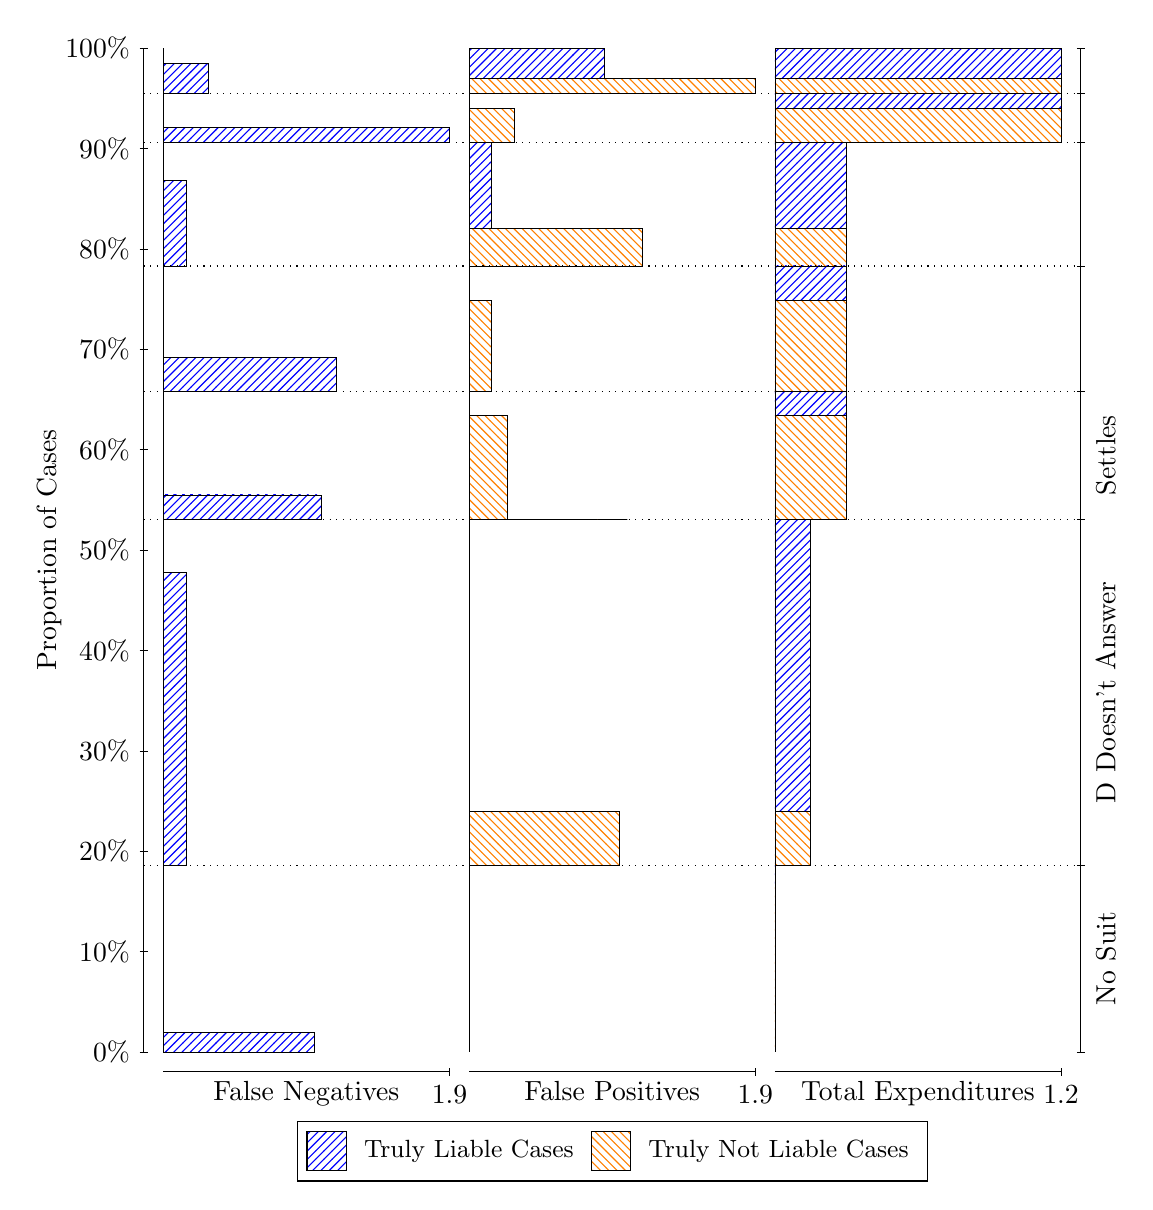
\begin{tikzpicture}
\draw[black, very thin] (1.5,1.75) -- (1.5,14.5);
\node[rotate=90, anchor=center] at (0.3, 8.125) {Proportion of Cases};
\draw[black, very thin] (1.45,1.75) -- (1.55,1.75);
\node[anchor=east] at (1.45, 1.75) {0\%};
\draw[black, very thin] (1.45,3.025) -- (1.55,3.025);
\node[anchor=east] at (1.45, 3.025) {10\%};
\draw[black, very thin] (1.45,4.3) -- (1.55,4.3);
\node[anchor=east] at (1.45, 4.3) {20\%};
\draw[black, very thin] (1.45,5.575) -- (1.55,5.575);
\node[anchor=east] at (1.45, 5.575) {30\%};
\draw[black, very thin] (1.45,6.85) -- (1.55,6.85);
\node[anchor=east] at (1.45, 6.85) {40\%};
\draw[black, very thin] (1.45,8.125) -- (1.55,8.125);
\node[anchor=east] at (1.45, 8.125) {50\%};
\draw[black, very thin] (1.45,9.4) -- (1.55,9.4);
\node[anchor=east] at (1.45, 9.4) {60\%};
\draw[black, very thin] (1.45,10.675) -- (1.55,10.675);
\node[anchor=east] at (1.45, 10.675) {70\%};
\draw[black, very thin] (1.45,11.95) -- (1.55,11.95);
\node[anchor=east] at (1.45, 11.95) {80\%};
\draw[black, very thin] (1.45,13.225) -- (1.55,13.225);
\node[anchor=east] at (1.45, 13.225) {90\%};
\draw[black, very thin] (1.45,14.5) -- (1.55,14.5);
\node[anchor=east] at (1.45, 14.5) {100\%};

\draw[black, very thin] (13.4,1.75) -- (13.4,14.5);
\draw[black, very thin] (13.35,1.75) -- (13.45,1.75);
\node[anchor=west] at (13.35, 1.75) {};
\draw[black, very thin] (13.35,4.1224) -- (13.45,4.1224);
\node[anchor=west] at (13.35, 4.1224) {};
\draw[black, very thin] (13.35,8.518) -- (13.45,8.518);
\node[anchor=west] at (13.35, 8.518) {};
\draw[black, very thin] (13.35,10.142) -- (13.45,10.142);
\node[anchor=west] at (13.35, 10.142) {};
\draw[black, very thin] (13.35,11.732) -- (13.45,11.732);
\node[anchor=west] at (13.35, 11.732) {};
\draw[black, very thin] (13.35,13.298) -- (13.45,13.298);
\node[anchor=west] at (13.35, 13.298) {};
\draw[black, very thin] (13.35,13.922) -- (13.45,13.922);
\node[anchor=west] at (13.35, 13.922) {};
\draw[black, very thin] (13.35,14.5) -- (13.45,14.5);
\node[anchor=west] at (13.35, 14.5) {};

\draw[black, very thin, pattern color=blue, pattern=north east lines] (1.75,1.75) rectangle (3.6623,1.9996);
\draw[black, very thin, pattern color=orange, pattern=north west lines] (1.75,1.9996) rectangle (1.75,4.1224);
\draw[black, very thin, pattern color=blue, pattern=north east lines] (1.75,4.1224) rectangle (2.0368,7.8394);
\draw[black, very thin, pattern color=orange, pattern=north west lines] (1.75,7.8394) rectangle (1.75,8.518);
\draw[black, very thin, pattern color=blue, pattern=north east lines] (1.75,8.518) rectangle (3.7579,8.8247);
\draw[black, very thin, pattern color=blue, pattern=north east lines] (1.75,8.8247) rectangle (3.5667,8.8247);
\draw[black, very thin, pattern color=blue, pattern=north east lines] (1.75,8.8247) rectangle (3.3754,8.8247);
\draw[black, very thin, pattern color=blue, pattern=north east lines] (1.75,8.8247) rectangle (3.1842,8.8247);
\draw[black, very thin, pattern color=blue, pattern=north east lines] (1.75,8.8247) rectangle (2.993,8.8247);
\draw[black, very thin, pattern color=blue, pattern=north east lines] (1.75,8.8247) rectangle (2.8018,8.8247);
\draw[black, very thin, pattern color=blue, pattern=north east lines] (1.75,8.8247) rectangle (2.6105,8.8247);
\draw[black, very thin, pattern color=blue, pattern=north east lines] (1.75,8.8247) rectangle (2.4193,8.8247);
\draw[black, very thin, pattern color=blue, pattern=north east lines] (1.75,8.8247) rectangle (2.2281,8.8247);
\draw[black, very thin, pattern color=orange, pattern=north west lines] (1.75,8.8247) rectangle (1.75,10.142);
\draw[black, very thin, pattern color=blue, pattern=north east lines] (1.75,10.142) rectangle (3.9491,10.576);
\draw[black, very thin, pattern color=orange, pattern=north west lines] (1.75,10.576) rectangle (1.75,11.732);
\draw[black, very thin, pattern color=blue, pattern=north east lines] (1.75,11.732) rectangle (2.0368,12.82);
\draw[black, very thin, pattern color=orange, pattern=north west lines] (1.75,12.82) rectangle (1.75,13.298);
\draw[black, very thin, pattern color=blue, pattern=north east lines] (1.75,13.298) rectangle (5.3833,13.49);
\draw[black, very thin, pattern color=orange, pattern=north west lines] (1.75,13.49) rectangle (1.75,13.922);
\draw[black, very thin, pattern color=blue, pattern=north east lines] (1.75,13.922) rectangle (2.3237,14.308);
\draw[black, very thin, pattern color=orange, pattern=north west lines] (1.75,14.308) rectangle (1.75,14.5);
\draw[black, very thin, pattern color=orange, pattern=north west lines] (5.6333,1.75) rectangle (5.6333,3.8728);
\draw[black, very thin, pattern color=blue, pattern=north east lines] (5.6333,3.8728) rectangle (5.6333,4.1224);
\draw[black, very thin, pattern color=orange, pattern=north west lines] (5.6333,4.1224) rectangle (7.5456,4.8009);
\draw[black, very thin, pattern color=blue, pattern=north east lines] (5.6333,4.8009) rectangle (5.6333,8.518);
\draw[black, very thin, pattern color=orange, pattern=north west lines] (5.6333,8.518) rectangle (7.6412,8.518);
\draw[black, very thin, pattern color=orange, pattern=north west lines] (5.6333,8.518) rectangle (7.45,8.518);
\draw[black, very thin, pattern color=orange, pattern=north west lines] (5.6333,8.518) rectangle (7.2588,8.518);
\draw[black, very thin, pattern color=orange, pattern=north west lines] (5.6333,8.518) rectangle (7.0675,8.518);
\draw[black, very thin, pattern color=orange, pattern=north west lines] (5.6333,8.518) rectangle (6.8763,8.518);
\draw[black, very thin, pattern color=orange, pattern=north west lines] (5.6333,8.518) rectangle (6.6851,8.518);
\draw[black, very thin, pattern color=orange, pattern=north west lines] (5.6333,8.518) rectangle (6.6851,8.518);
\draw[black, very thin, pattern color=orange, pattern=north west lines] (5.6333,8.518) rectangle (6.4939,8.518);
\draw[black, very thin, pattern color=orange, pattern=north west lines] (5.6333,8.518) rectangle (6.3026,8.518);
\draw[black, very thin, pattern color=orange, pattern=north west lines] (5.6333,8.518) rectangle (6.1114,9.8349);
\draw[black, very thin, pattern color=blue, pattern=north east lines] (5.6333,9.8349) rectangle (5.7289,9.8349);
\draw[black, very thin, pattern color=blue, pattern=north east lines] (5.6333,9.8349) rectangle (5.6333,10.142);
\draw[black, very thin, pattern color=orange, pattern=north west lines] (5.6333,10.142) rectangle (5.9202,11.297);
\draw[black, very thin, pattern color=blue, pattern=north east lines] (5.6333,11.297) rectangle (5.6333,11.732);
\draw[black, very thin, pattern color=orange, pattern=north west lines] (5.6333,11.732) rectangle (7.8325,12.209);
\draw[black, very thin, pattern color=blue, pattern=north east lines] (5.6333,12.209) rectangle (5.9202,13.298);
\draw[black, very thin, pattern color=orange, pattern=north west lines] (5.6333,13.298) rectangle (6.207,13.73);
\draw[black, very thin, pattern color=blue, pattern=north east lines] (5.6333,13.73) rectangle (5.6333,13.922);
\draw[black, very thin, pattern color=orange, pattern=north west lines] (5.6333,13.922) rectangle (9.2667,14.113);
\draw[black, very thin, pattern color=blue, pattern=north east lines] (5.6333,14.113) rectangle (7.3544,14.5);
\draw[black, very thin, pattern color=orange, pattern=north west lines] (9.5167,1.75) rectangle (9.5167,3.8728);
\draw[black, very thin, pattern color=blue, pattern=north east lines] (9.5167,3.8728) rectangle (9.5167,4.1224);
\draw[black, very thin, pattern color=orange, pattern=north west lines] (9.5167,4.1224) rectangle (9.9708,4.8009);
\draw[black, very thin, pattern color=blue, pattern=north east lines] (9.5167,4.8009) rectangle (9.9708,8.518);
\draw[black, very thin, pattern color=orange, pattern=north west lines] (9.5167,8.518) rectangle (10.425,8.518);
\draw[black, very thin, pattern color=blue, pattern=north east lines] (9.5167,8.518) rectangle (10.425,8.518);
\draw[black, very thin, pattern color=orange, pattern=north west lines] (9.5167,8.518) rectangle (10.425,9.8349);
\draw[black, very thin, pattern color=blue, pattern=north east lines] (9.5167,9.8349) rectangle (10.425,10.142);
\draw[black, very thin, pattern color=orange, pattern=north west lines] (9.5167,10.142) rectangle (10.425,10.142);
\draw[black, very thin, pattern color=blue, pattern=north east lines] (9.5167,10.142) rectangle (10.425,10.142);
\draw[black, very thin, pattern color=orange, pattern=north west lines] (9.5167,10.142) rectangle (10.425,11.297);
\draw[black, very thin, pattern color=blue, pattern=north east lines] (9.5167,11.297) rectangle (10.425,11.732);
\draw[black, very thin, pattern color=orange, pattern=north west lines] (9.5167,11.732) rectangle (10.425,12.209);
\draw[black, very thin, pattern color=blue, pattern=north east lines] (9.5167,12.209) rectangle (10.425,13.298);
\draw[black, very thin, pattern color=orange, pattern=north west lines] (9.5167,13.298) rectangle (13.15,13.73);
\draw[black, very thin, pattern color=blue, pattern=north east lines] (9.5167,13.73) rectangle (13.15,13.922);
\draw[black, very thin, pattern color=orange, pattern=north west lines] (9.5167,13.922) rectangle (13.15,14.113);
\draw[black, very thin, pattern color=blue, pattern=north east lines] (9.5167,14.113) rectangle (13.15,14.5);
\draw[black, dotted] (1.5,4.1224) -- (13.4,4.1224);
\draw[black, dotted] (1.5,8.518) -- (13.4,8.518);
\draw[black, dotted] (1.5,10.142) -- (13.4,10.142);
\draw[black, dotted] (1.5,11.732) -- (13.4,11.732);
\draw[black, dotted] (1.5,13.298) -- (13.4,13.298);
\draw[black, dotted] (1.5,13.922) -- (13.4,13.922);
\draw[black, very thin] (1.75,1.5) -- (5.3833,1.5);
\node[anchor=north] at (3.5667, 1.5) {False Negatives};
\draw[black, very thin] (5.3833,1.45) -- (5.3833,1.55);
\node[anchor=north] at (5.3833, 1.45) {1.9};

\draw[black, very thin] (5.6333,1.5) -- (9.2667,1.5);
\node[anchor=north] at (7.45, 1.5) {False Positives};
\draw[black, very thin] (9.2667,1.45) -- (9.2667,1.55);
\node[anchor=north] at (9.2667, 1.45) {1.9};

\draw[black, very thin] (9.5167,1.5) -- (13.15,1.5);
\node[anchor=north] at (11.333, 1.5) {Total Expenditures};
\draw[black, very thin] (13.15,1.45) -- (13.15,1.55);
\node[anchor=north] at (13.15, 1.45) {1.2};

\node[black, centered, rotate=90] at (13.72, 2.9362) {No Suit};
\node[black, centered, rotate=90] at (13.72, 6.3202) {D Doesn't Answer};
\node[black, centered, rotate=90] at (13.72, 9.3298) {Settles};





\draw (7.449999999999999,1.5) node[draw=none] (baseCoordinate) {};
\begin{scope}[align=center]
        \matrix[scale=0.5, draw=black, below=0.5cm of baseCoordinate, nodes={draw}, column sep=0.1cm]{
            \node[rectangle, draw, minimum width=0.5cm, minimum height=0.5cm, pattern=north east lines, pattern color=blue] {}; &
            \node[draw=none, font=\small] (B) {Truly Liable Cases}; &
            \node[rectangle, draw, minimum width=0.5cm, minimum height=0.5cm, pattern=north west lines, pattern color=orange] {}; &
            \node[draw=none, font=\small] (B) {Truly Not Liable Cases}; \\
            };
\end{scope}

\end{tikzpicture}
\end{document}